\section[Využití iontových svazků v materiálovém výzkumu]{Využití iontových svazků v materiálovém výzkumu: Základní typy urychlovačů, Metody RBS, kanálování, PIXE, PIGE, ERDA a NRA}

\subsection{Základní typy urychlovačů}

\textbf{Definice:} Urychlovač je zařízení, které umožňuje zvýšení kinetické energie nabité (urychlované) částice, a to pomocí elektrické pole, které může být statické nebo proměnně a přitom je vede po stanovené trajektorii, a to pomocí megnetického pole, jež může být opět statické a nebo proměnné. Urychlovat lze pouze nabité částice, stejně tak jako je vést po určité dráze vlivem magnetického/elektromagnetického pole.

Díky případnému konverznímu materiálu lze eventuelně převést nabité částice na jiný typ záření (neutrony, fotony).

\textbf{Základní komponenty urychlovače:}

\begin{itemize}
    \item Zdroj nabitých částic
    \item Urychlovací trubice (EM pole)
    \begin{itemize}
        \item VN zdroj vytvářecí urychlovací napětí a magnety v urychlovačí (dipóly = zakřivení dráhy pohybu částic, kvadrupóly = fokusace svazku).
    \end{itemize}
    \item Systém dodávky EM polí
    \item Extrakce urychlených částic z urychlovače a soustředění na terčík
    \item Bombardovaný terčík a detektor/y pro popis parametrů urychleného svazku
    \item Diagnostika svazku (sledování energie, intenzity, polohy)
    \item Systém napájení
    \item Řídicí systém
    \item Vakuový systém
\end{itemize}

\textbf{Rozdělení:}

\begin{itemize}
    \item Dle trajektorie -- Dle trajektorie rozdělujeme urychlovače na lineární (elektrostatické vs. rezonanční, pro konstantní vs. proměnné urychlovací napětí) a cyklické (mikrotron, betatron, cyklotron, synchrotron, synchocyklotron, izochronní cyklotron).
    \item Dle způsobu urychlení -- Dle způsobu urychlení rozdělujeme Elektrostatické a Rezonanční, což je například pro lineární urychlovače velmi efektivní a jsme schopni získat jednotky až desítky MeV na jednotkách metrů (1 m je cca jednotky až destíky MeV).
    \item Dle režimu práce -- Kontinuální (časově neměnný svazek) a Impulzní (uvolňování částic po částech/balících).
\end{itemize}

\textbf{Princip urychlení a zakřivení}:

Velmi to záleží jestli mám cyklický a nebo lineární a pak podle typu napětí EM pole.

\begin{itemize}
    \item Lineární elektrostatický $\rightarrow$ v tomto případě mám rovnou trubici, kde mám dáno urychlovací napětí konstatní a částice je na dáne dráze urychlena tak moc, jak je dáno napětí. Magnetické pole pak zde slouží v podobě dipólů nebo kvadrupólů, a to pro korekci svazku, aby se nevychyloval a pro jeho fokusaci. K tomu se pak typicky ale využívá tzv. elektrostatický fokusační systém, který je tvořen 4 elektrodami, jež jsou vždy 2 a 2 naproti sobě se stejným napětím a způsobují, že částice je "odrážena" doprostřed.
    \item Lineární rezonanční $\rightarrow$ Přímočará dráha pohybum proměnlivý proud (napětí se cyklicky mění a jednotlivé elektrody mění náboj, aby buď odpuzovaly či přitahovaly), zvětšující se délka urychlovacích segmentů s délkou (částice se hýbe velmi rychle, tak to musí mít nějaký efekt a aby ji to vůbec stihlo urychlit, tak jsou delší a delší). Hodně se to využívá v medicíně, protože na krátké vzdálenosti naberou částice vysokou energii a poté se využívá např. převod elektronu na RTG či $\gamma$. V klidu se dá urychlit na 10-15 MeV/m
    \item Cyklický (konst. napětí i magnetické pole) $\rightarrow$ V tomto případě přiletí částice a urychlovacím napětím jí roste energie a magnetickým polem je zakřivena její dráha pohybu, která se s jeho konstatností zvětšuje v poloměru. Celý urychlovač je navržen tak, že při správné energii dosáhne částice maximálního poloměru dráhy pohybu a vyletí ústím ven.
    \item Cyklický (konst. napětí) $\rightarrow$ Stejné jako výše, avšak pomocí proměnlivého magnetického pole mohu částici udržovat na stejném poloměru zakřivení.
    \item Cyklický (obojí proměnlivé) $\rightarrow$ Mám tam například místa, kde když částice projde, tak ji to urychlý a stejně jako u lineárního dochází k periodickému přepólování, aby částice byla odpuzována/přitahována ve správný moment. Proměnlivým magnetickým polem je pak držena na stejném poloměru.
\end{itemize}

\textbf{Využití:} Materiálový výzkum, částicová fyzika, Produkce radionuklidů (do medicíny či materiálový výzkum), Produkce neutronů (studium radiačního poškození, difrakce neutronů, neutronová fyzika, produkce fotonů (materiálový výzkum-XFEL a medicína).

\subsection{Metoda RBS}

= Rutherford Backscatterring Spectroscopy

Využití pružného rozptylu nalétávajících iontů z monoenergetického svazku (E=1-3 MeV) s atomy či jejich elektrony v terčíku.

\begin{itemize}
    \item Pružný rozptyl = bez ztráty energie na srážku
    \item Měření počtu a energii odražených iontů dopadajícího svazku, což nám dává info o materiálu terčíku.
    \item Typické hloubky, kde je RBS schopno identifikovat a lokalizovat různé prvky v matrici jsou desítky až stovky nm.
\end{itemize}

\textbf{Výhody:}

\begin{itemize}
\item vysoká citlivost na těžké prvky v lehké matrici
\item jednoduché umístění vzorku na vzduchu
\item kvalitativní přesnost < 1 \%
\item hloubkové rozlišení < 5 nm se Si(Li) detektorem
\item kanálování
\item Vysoká přesnost na těžké prvky v lehké matrici
\item Schopnost velmi dobře rozlišit dva lehké prvky mezi sebou navzájem (dva lehké prvky s malým rozdílem hmotnosti), a to např. O-18 a F-19, C-13 a N-14
\end{itemize}

\textbf{Nevýhody:}

\begin{itemize}
\item necitlivé na lehké prvky v těžké matrici
\item implantování iontů do analyzovaného materiálu
\item potřebný urychlovač
\item Problém rozlišit dva těžké prvky o podobné hmotnosti (Pb-208 a Au-197), avšak rozlišovací schopnost lze zlepšit zvýšením hmotnosti dopadající částice ($M_1$) $~rightarrow$ citlivost při dopadu alfa částice je lepší v porovnání s protony.
\end{itemize}

\begin{figure}[H]
    \centering
	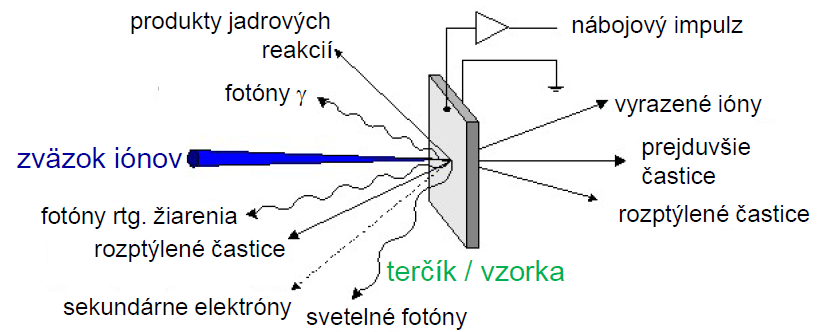
\includegraphics[width=10cm]{img/iont-svazky.png}
	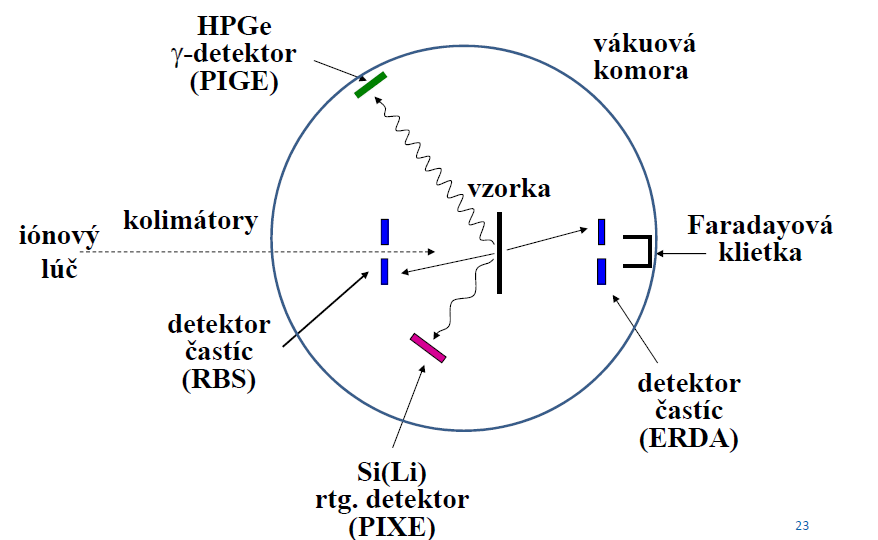
\includegraphics[width=7cm]{img/iont-svazky-exp.png}
\end{figure}

V zásadě existují dva procesy, resp. interakce urychlených iontů s danou látkou:

\textbf{1) Interakce s jádrem (Elastický Coulombův rozptyl):}

\begin{itemize}
    \item Víme počáteční energii $E_0$, víme jeho hmotnost $M_1$ a měříme jeho energii $E_1$ po jeho zpětném rozptylu.
    \item Využijeme $E_1$ = K * $E_0$, kde K je kinematický faktor a je funkcí hmotností obou interagujících částic a úhlu odrazu zaznamenáného odraženého iontu
    \item Neznámou tedy představuje pouze hmotnost $M_2$, kterou jsme schopni z toho dopočítat a určit o jaké jádro se jedná.
\end{itemize}

\textbf{2) Interakce s elektrony (elektronový rozptyl):}

\begin{itemize}
    \item Lokalizace a určení atomu ($M_2$) jakožto funkce hloubky, resp. v závislosti na tom v jaké hloubce dojde k rozptylu.
    \item množství úbytku energie záleží na brzdném účinku látky, tedy na hustotě elektronů v látce a vzdálenosti, kterou nabitý iont urazí při průchodu látkou.
    \item Prvky, které se v materiálu objevují pouze v určité hloubce mají na naměřeném spektru svůj pík posunuty, ale jsou posunuty o jistou míru/energii, která představuje vzdálenost, kterou musel iont projít materiálem, aby se k nim dostal.
    \item Ke stanovení je nutné mít naměřenou energii iontu po odrazu na povrchu a pak následně v dané hloubce. Čím hlouběji iont musel jít, tím více ztratí energie
    \item Správnost určení rozdílu energií při odrazu na povrchu a v hloubce ($\Delta E$) závisí na = energetické rozlišení detektoru, energetický rozptyl urychleného svazku dopadajících iontů a také energetický rozptyl směrem k a od terčíku, příprava povrchu terčíku. Na závěr samozřejmě závisí na materiálu, který je měřen.
\end{itemize}

\textbf{Měřené spektrum podle tloušťky měřeného vzorku materiálu:}

\begin{itemize}
    \item Ultra tenká vrstva (několik atomárních vrstev)
    \begin{figure}[H]
        \centering
        \includegraphics[width=0.5\linewidth]{img/ultra tenká vrstva - RBS.png}
        \caption{ultra tenká vrstva -- RBS}
    \end{figure}

    \item Tenká vrstva (několik stovek až tisíců atomárních vrstev)

    \begin{figure}[H]
        \centering
        \includegraphics[width=0.5\linewidth]{img/Tenká vrstva - RBS.png}
        \caption{Tenká vrstva -- RBS}
    \end{figure}

    \item Hrubá vrstva = toto už jsou mm, v zásadě bulk/objem.

    \begin{figure}[H]
        \centering
        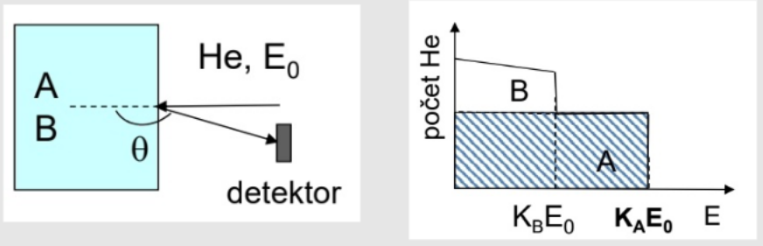
\includegraphics[width=0.5\linewidth]{img/Bulk - RBS.png}
        \caption{Bulk -- RBS}
    \end{figure}

    \item Pokrytí povrchu = bulk materiál, který má na povrchu naneseny různé tloušťky jiného materiálu/materiálů. Zde rozdělujeme 2 varianty (lehký bulk a těžké pokrytí a naopak)

    \begin{figure}[H]
        \centering
        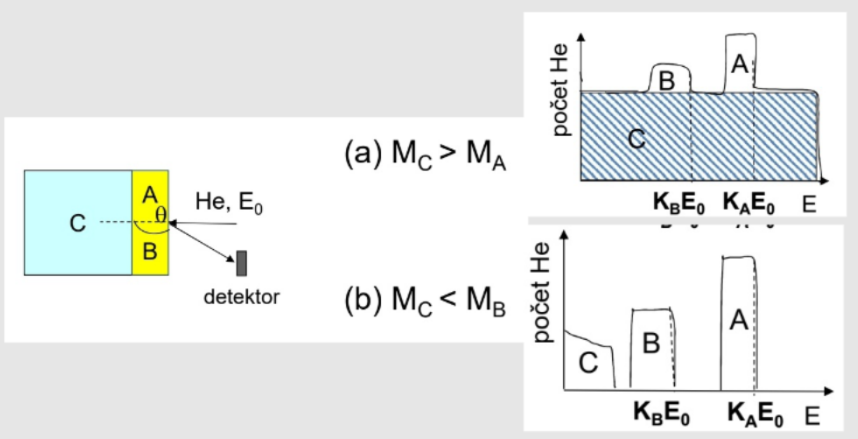
\includegraphics[width=0.5\linewidth]{img/pokrytí - RBS.png}
        \caption{Pokrytí -- RBS}
    \end{figure}
\end{itemize}

\textbf{Kvalitativní analýza:}

\begin{figure}[H]
    \centering
	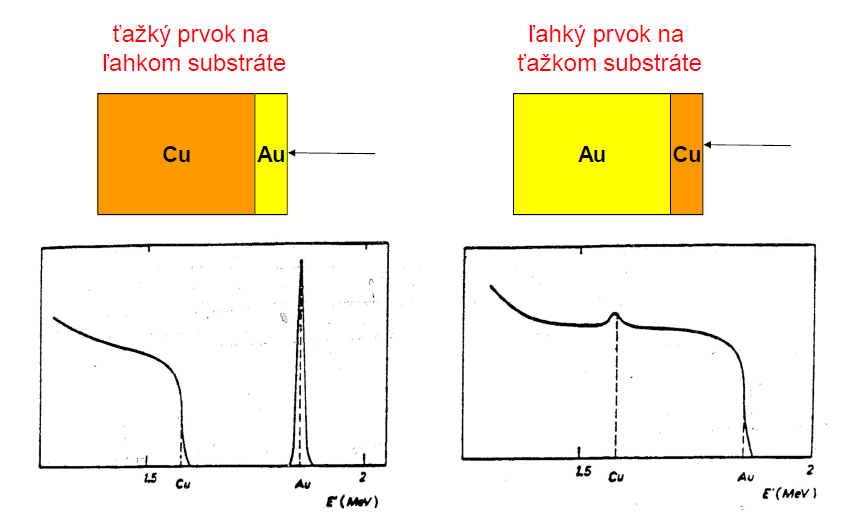
\includegraphics[width=9cm]{img/rbs-analyza.png}
	%	\includegraphics[width=7cm]{rbs2.png}
	%	\includegraphics[width=7cm]{rbs3.png}
\end{figure}

Výstupem při měření dostáváme z detektoru impulsy, jejichž výška je úměrná energii zpětně odraženého iontu. Z výšky čar výsledného spektra lze stanovit stechiometrické složení vzorku.

\textbf{Využití:}

Detektory částic nastavené na RBS jsou často součásti většího celku jehož součásti jsou i detektory na PIGE, PIXE, ERDA a celé to bývá vaukováno, aby nedocházelo k parazitní interakci s částicemi atmosféry (nahoře je ovšem psáno, že RBS jde dělat i na vzduchu, což jde, ale je lepší tam tu parazitní interakci nemít).

Umění, archeologie (sochy, obrazy, předměty -- například rozdíl mezi zlatem a pozlacením), materiálový výzkum a geologie.

\subsection{Kanálování}

Kanálování je speciální mód RBS techniky. Vyžadováno je, aby orientace urychlených iontů byla ve správné poloze vůči krystalografické mříži, a to konkrétně podél hlavní krystalografické osy krystalu.

V čistém a ideálním krystalu by měl iont jakoby "projít rovně skrz  a mezi jednotlivými rovinami", avšak v případě přítomnosti poruch či příměsí jsme schopni detekovat jejich polohu v krystalu, jelikož pak dochází k poklesu intenzity detekovaného záření (stínení Coulombovského rozptylu).

\begin{figure}[H]
    \centering
	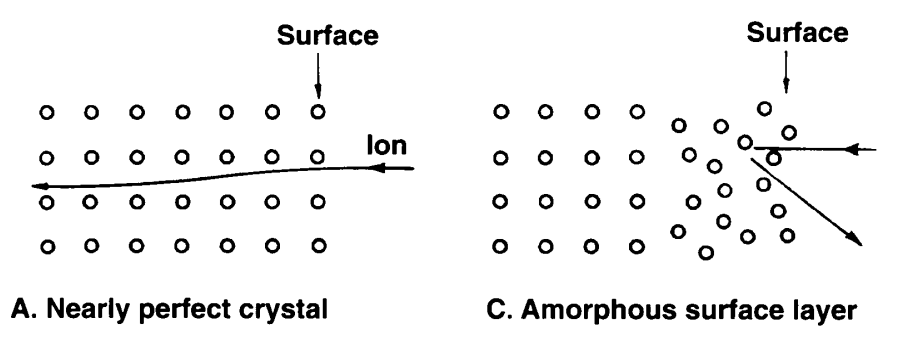
\includegraphics[width=10cm]{img/rbs-kanalovani.png}
	%	\includegraphics[width=7cm]{rbs2.png}
	%	\includegraphics[width=7cm]{rbs3.png}
\end{figure}

\subsection{PIXE}

= Particle Induced X-Ray Emission

Jedná se nedestruktivní o metodu, která využívá detekce charakteristického RTG záření.

\textbf{Výhody:}

\begin{itemize}
    \item Nedestruktivní technika schopna měřit tuhé látky, tekutiny i aerosoly
    \item Vysoká citlivost a rychlost měření
    \item Dobrá rozlišovací schopnost = multiprvková analýza (Z > 13 = Al)
\end{itemize}

\textbf{Nevýhody:}

\begin{itemize}
    \item Nelze analyzovat organické vzorky
    \item Omezená hloubková informace
    \item Potřeba urychlovače
\end{itemize}

\textbf{Princip:}

Excitací atomu iontovým svazkem (vyražení elektronu a jeho zabrání elektronem z vyšší energetické hladiny) a produkce charakteristického RTG záření, jehož detekči lze identifikovat původce a identifikovat tak prvek (v zásadě stejné jako u RFA, akorát tady se využívají ionty a ne fotony z radionuklidu nebo rentgenky).

Stejně jako u RFA, tak i zde je Augerův elektron konkurenční jev a dohromady dávají jedničku. Takže existuje klasicky pravděpodobnost, že k vyzáření RTG dojde a ta je dána účinným průřezem pro ionizaci a fluorescenčním výtěžkem.

Stejně jako u RFA, tak se projevují matricové jevy, které mi ovlivňují měření, tedy to co naměřím a to co realně je ve zkoumaném materiálu.

Stejně jako u RFA, tak plocha pod čarou je rovna koncentraci prvku

K detekci charakteristického RTG záření se využívá HPGe, Si(Li)

\begin{figure}[H]
    \centering
	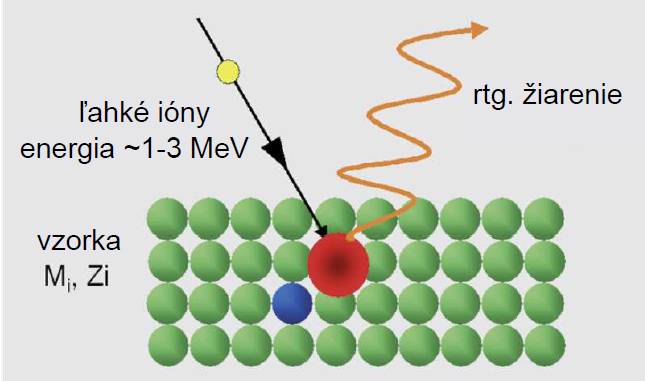
\includegraphics[width=8cm]{img/pixe.png}
	%	\includegraphics[width=7cm]{rbs2.png}
	%	\includegraphics[width=7cm]{rbs3.png}
\end{figure}

\textbf{Aplikace a využití:}

\begin{itemize}
    \item Materiálový výzkum
    \item Geologie
    \item Umění, architektura
    \item Monitoring znečištění atmosfŕy
\end{itemize}

\textbf{Speciální případy:}

\begin{itemize}
    \item Mikrosvazek = distribuce prvků ve vzorku (analýza hrubých vrstve s vysokým rozlišením) $\rightarrow$ stopová množství, malé oblasti s vysokým rozlišením.
    \item Externí svazek = Analýza velkých a komplexních předmětů svazkem z urychlovače, který je vyveden ven do atmosféry na zkoumaný objekt (proto externí svazek)$\rightarrow$ Louvre, artefakty, obrazy.
\end{itemize}

\subsection{PIGE}

=Particle Induced Gamma Emission

Jedná se o nedestruktivní metodu pro stanovení prvkového složení na základě interakce urychlených protonů, popř. d, $\alpha$ a málokdy těžkých iontů s jádrem atomu za vzniku gama záření, které poté detekujeme. Toto záření tak je pak v některých případech doprovázeno ještě další reakcí, resp. vznikem další částice/záření.

Nejčastěji se opět měří ve vakuové komoře a nejvíce se využívají urychlené protony.

\begin{itemize}
    \item Rezonanční záchyt (p, $\gamma$) - mohu využít rezonancí prvků, které jsou ve zkoumaném materiálu a pak detekuji jen gamu. To ale vyžaduje, že vím co tam je, resp. vím co v tom hledám, abych danou rezonanci mohl využít.
    \item nepružný záchyt (p, $p^| \gamma$)
    \item Srážky s přeuspořádáním (p, n$\gamma$), (p, $\alpha\gamma$), (p,n)
\end{itemize}

\subsection{ERDA}

=Elastic Recoil Detection Analysis

Jedná se o metodu využívající pružný rozptyl lehkých jader po dopadu těžkých iontů. Slouží pro detekci lehkých prvků v těžké matrici (dokáže detekovat vodík v tuhých látkách)

\textbf{Výhody:}

\begin{itemize}
    \item Dobrá citlivost na lehké prvky.
    \item Dá se kombinovat s RBS.
    \item Menší poškození vyšetřovaného materiálu.
    \item Idektifikace 1-H a 2-H hloubkových profilů (pomocí alfa).
\end{itemize}

\textbf{Nevýhody:}

\begin{itemize}
    \item Menší hloubkové rozlišení a hloubka analýzy (způsobeno hmotností, resp. velikosti těžších iontů) je kvůli rozptylu dopadajících iontů asi několik stovek nm.
    \item Vzorek musí být spešl připraven + omezená geometrie ozařování a detekce.
\end{itemize}

\textbf{Princip:}

Pružný rozptyl dopadajícíh vysokoenergetických a těžkých iontů (MeV), ven jdou odražené ionty a vyražené atomy z materiálu

Umožňuje profilování lehkých jader.

S využitím standardů umožňuje i kvantitativní analýzu.

\begin{figure}[H]
    \centering
	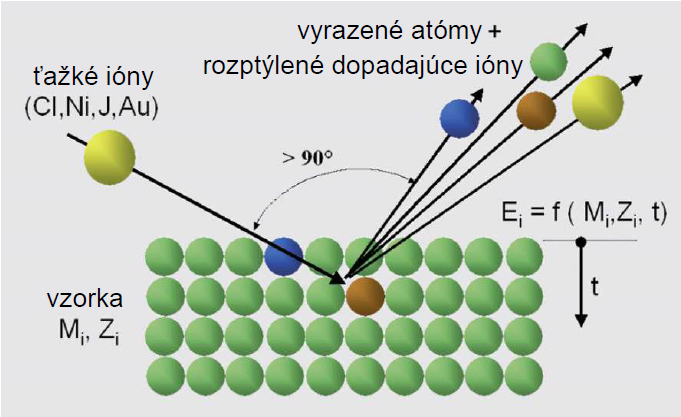
\includegraphics[width=8cm]{img/erda.png}
	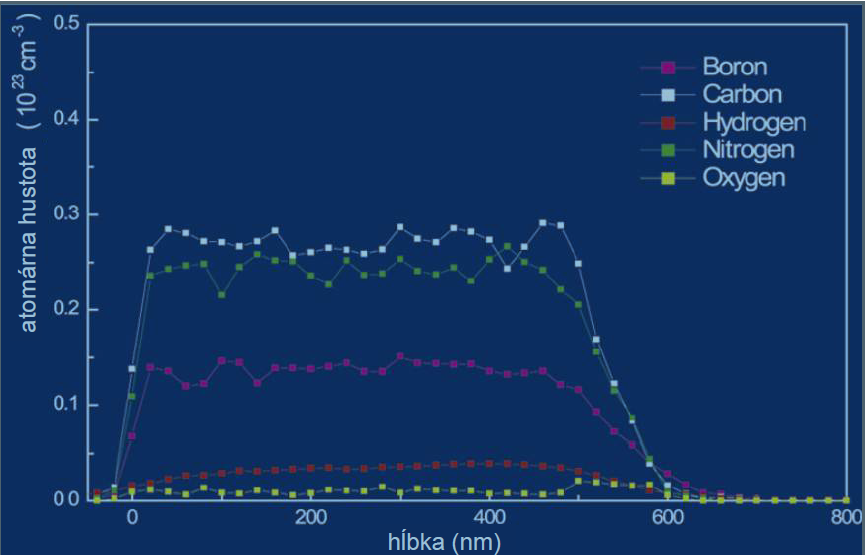
\includegraphics[width=7cm]{img/erda-spektrum.png}
	%	\includegraphics[width=7cm]{rbs3.png}
\end{figure}

\textbf{Módy provozu:}

\begin{itemize}
    \item Transmisní: Velmi tenké vzorky
    
    \begin{figure}[H]
        \centering
        \includegraphics[width=0.38\linewidth]{img/transmisní ERDA.png}
        \caption{transmisní ERDA}
    \end{figure}

    \item Odraz pod malými úhly = nejčastější metoda

    \begin{figure}[H]
        \centering
        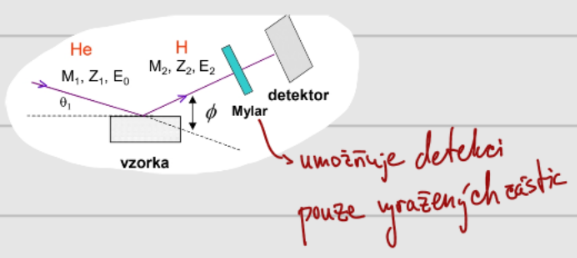
\includegraphics[width=0.5\linewidth]{img/odrazová ERDA.png}
        \caption{odrazová ERDA}
    \end{figure}
\end{itemize}

V obou geometriích platí, že $E_2 = K * E_0$, kde faktor $K$ závisí na hmotnostech bombradující a vyražené částice a dále na úhlu rozptylum takže pak jen určíme zase hmotnost $M_2$.

\subsection{NRA}

= Nuclear Reaction Analysis

Jedná se o metodu pro detekci lehkých prvků (Z < 18), jež je izotopicky citlivá a umožňuje identifikaci a lokalizaci stopových prvků. Jedná se o nedestruktivní metodu s analytickou hloubkou několik stovek nm, ovšem jedná se vždy o exotermickou nebo endotermickou reakci a tudíž energetická bilance je vždy nenulová.

Jedná se o nepružný proces, a proto se částice na začátku nerovnají produktům reakce.

\textbf{Princip:}

Jaderná reakce mezi dopadajícím iontem a prvkami v terčíku. Následně dochází k detekci produktů reakce ($\gamma$ nebo částice).

\begin{figure}[H]
    \centering
	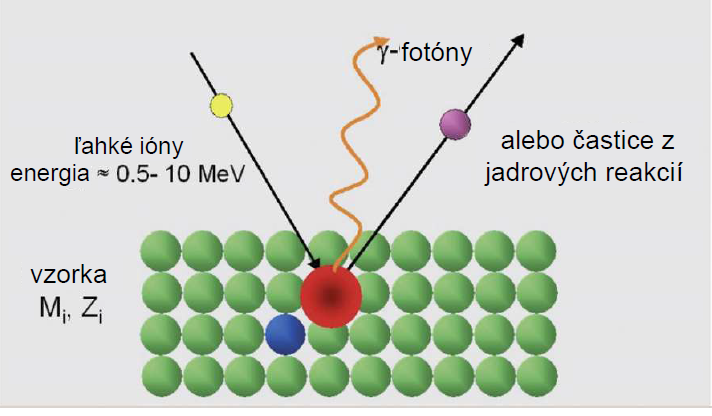
\includegraphics[width=8cm]{img/nra.png}
	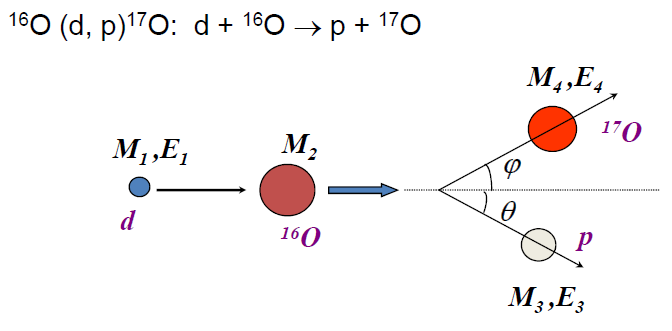
\includegraphics[width=7cm]{img/nra2.png}
	%	\includegraphics[width=7cm]{rbs3.png}
\end{figure}

Detekuji produkty reakce (částice nebo $\gamma$)( pomocí Si detektoru nebo $\gamma$ fotony detekuju pomocí Ge či NaI(Tl) detektorů)a změřím si energii $E_3$ pro dané $M_1$, $E_1$ a $\theta$ a tím identifikuji $M_2$.

Poté si naměřím spektrum $E_3$, které mi podá informaci o hloubkovém rozložení $M_2$ a tím ho lokalizuji v materiálu.


\textbf{Pozn.:} Reakce může probíhat dvojím způsobem, a to sice přes složené jádro (všechny nukleony jsou využity) a nebo jakožto tzv. přímá reakce, kde jen některé nukleony jsou použité (někdy nazýváno trhací reakce).

Pravděpodobnost reakce je klasicky dána příslušným účinným průřezem.

K detekci příslušných jader v hloubce nebo na povrchu se dají využít rezonance, kdy pokud se energie bombardující částice rovná energii rezonance, tak k interakci dojde na povrchu. Pokud je ovšem energie částice vyšší než energie rezonance, tak k interakci dojde v hloubce pod povrchem (cestou do materiálu se energie sníží a až se vyrovná tak interaguje).

Příkladem je analýza vodíku pomocí 15-N za vzniku 12-C + 4-He a $\gamma$. Rezonance je při 6,385 MeV a s hloubkou dochází k posuvu rezonance, a proto se vyuźívájí energie vyšší než rezonance až napŕ. do 15 MeV.

\textbf{Využití:} Farmacie, archeologie, Geovědy, umění

\textbf{Srovnání RBS a NRA:}

\begin{itemize}
    \item RBS je pro detekci těžkých prvků v lehké matrici, zatímco NRA je pro detekci lehkých prvků.
    \item RBS využívá elastický rozptyl dopadajících částic (typicky $\alpha$ = 2 MeV), zatímco NRA vyuźívá nepružný roztpyl mezi dopadající částicí a částicí v terčíku (detekce produktů reakce)
    \item RBS má energetickou bilanci nulovou a NRA nemá
    \item u RBS jsou jádra terčíku i dopadající částice v základním stavu, zatímco u NRA jsou produkty reakce odlišné od původních, které do reakce vstupují.
\end{itemize}